\en

\section{Tool architecture}
\label{subsec:architecture}

The Setup step consists of two components, the Function Breaker and the Code Duplication Finder. 
The pipeline of this step works as follows: the Function Parser receives the codebase the user 
is interested in, extracts the functions of the codebase along with metadata, and creates a new 
temporary codebase where the functions extracted become news code files. The Code Duplication Finder 
iterates over every pair of files in the temporary codebase, checks if they are code clones, and if 
so, saves them in the Code Duplication Database, which is a text file that stores every code duplication 
as a triple \textbf{<function1,function2,similarity>}, where function1 and function2 are the functions 
that are a duplication of each other, the similarity is the metric given by the code duplication detection 
method utilized, which in our case, it is the cosine similarity explained in \ref{sec:similarity}. 
Finally, the Query Responder consumes the temporary codebase and the Code Duplication Database to 
extract duplicated functions-related information per user request. Figure \ref{fig:diagram} illustrates 
the tool pipeline. There is an explanation of how each component works through this section.

\begin{figure}
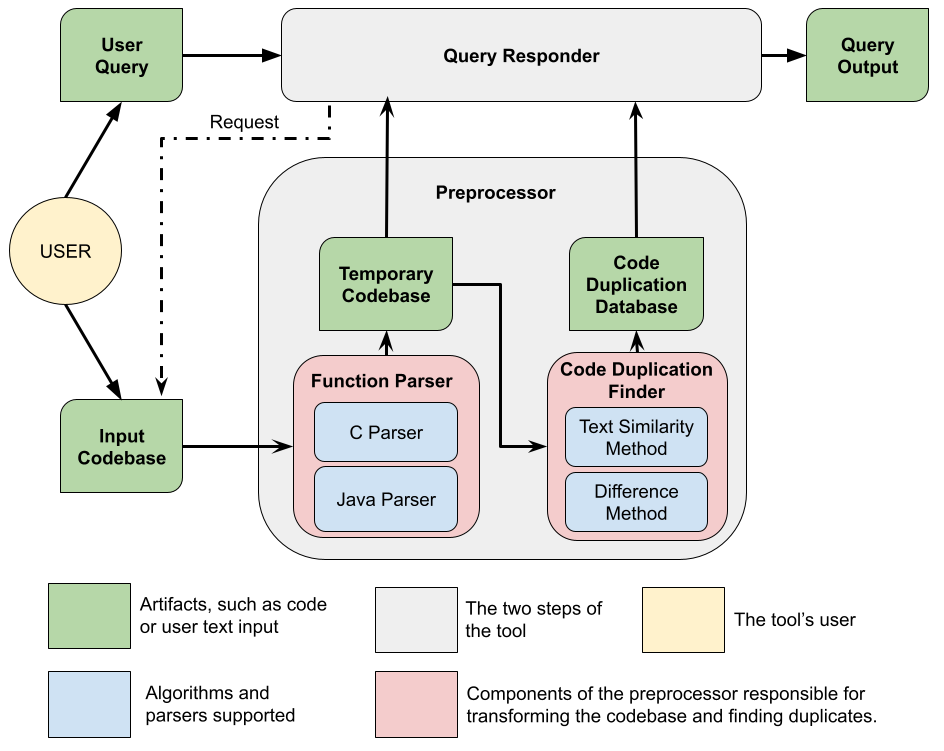
\includegraphics{diagrama_mestrado}
\caption{The architecture diagram demonstrating the relationship between the tool components.}
\label{fig:diagram}
\end{figure}

\subsection{Input codebase}

The input codebase is a folder in the machine the tool is running into. All files in the codebase 
that are not source code files from a supported programming language by the tool are ignored. The 
tool validates the support for a source file through analysis of its file extension.

\subsection{Function Parser}

The Function Parser receives the input codebase and transforms it into the temporary codebase. The 
Function Parser iterates through every source code file from the programming language it supports 
and uses a specific programming language function extractor to extract every function in the file. 
For each function extracted, we create two new source code files and a metadata file in the temporary 
codebase, represented by the pair,  the source code file of the function, and the proper function. 
The first new source code file contains the function’s body from the function it represents, while 
the other new source code file contains the function’s signature. The metadata file contains 
additional relevant information about the function, such as the function name, the line where the 
function signature starts in the source code file, and the line where the function’s body ends in 
the source code file. The programming language we support at the moment is C and Java. Can be found 
an example of a transformation of a source code in Figure (CREATE FIGURE AND ADD HERE).

About the programming language’s function extractor, we approached this problem in a way that any 
person comfortable with a language can adapt our approach to their specific programming language. 
Usually, the code blocks can be easily extracted from source code files, independently if the code 
blocks are defined by curly brackets or by indentation, and it is possible to infer if it represents 
a function’s body given how deeply it is in the code context and a few lines before the start of the 
code block. We followed this approach to implement the function extractor for the supported languages. 
As an alternative approach, we can build the syntax tree \citep{compiler} 
of the programming language and use it to extract the functions, which is a more complex task than 
our approach. For the programming languages that we support, we implemented them as follows:

\begin{itemize}
	\begin{item}
		\textbf{C}: Given a source code file, we extract every code block from it, maintaining the depth 
		of the code block in the code context and some of the code lines before the definition of the 
		code block. According to the C programming language’s grammar, functions are defined in a 
		global context at depth 0. There are other elements with the same depth as functions, and we 
		differentiate them by analyzing if the first non-empty character before the curly brackets of 
		the code block is a closing parenthesis. This pattern uniquely identifies functions 
		within C code.

	\end{item}
	\begin{item}
		\textbf{Java}:  Given a source code file, we extract every code block from it, maintaining the 
		depth of the code block in the code context and some of the code lines before the definition 
		of the code block. According to Java’s grammar, the functions are defined inside classes. 
		Functions can exist in different depths, as Java accepts inner classes. We differentiate 
		functions of other elements by analyzing if the first non-empty character before the curly 
		brackets of the code block is a close parenthesis. There is a problem with this approach in 
		Java, as there are other elements that respect this pattern, such as for loop, thus requiring 
		more filters. We chose to analyze functions of depth 1, which ignores every other element that 
		is a code block and has a parenthesis as the first non-empty character before the curly brackets. 
		The counterpart to this choice is that the extractor does not find functions declared inside 
		inner classes. The counterpart is not a problem in this work as there are no inner classes 
		on the BigCloneBench \citep{bigclonebench}, the only codebase in Java explored in this work.

		
	\end{item}
\end{itemize}

\subsection{Temporary codebase}

The temporary codebase is a transformation of the input codebase done by the Function Parser. 
Each function in the input codebase is represented in the temporary codebase as three files.
Descriptions of these files are provided below, and an example of each can be found in 
the figure (CREATE FIGURE AND ADD HERE).

\begin{itemize}
	\begin{item}
		\textbf{Header file}: This file contains the signature of the function it represents;
	\end{item}
	\begin{item}
		\textbf{Source file:} This file contains the body of the function it represents;
	\end{item}
	\begin{item}
		\textbf{Info file:} This file contains metadata of the function. The information this 
		file contains is the function name, the file that has the function, the relative path 
		of the file related to the input codebase, the line that the function’s signatures 
		start, the line that the function body initiates, the line that the function’s body 
		ends and if there is a line break between the end of the function’s signature and the 
		start of the function’s body.
	\end{item}
\end{itemize}

\subsection{Code Duplication Finder}

The Code Duplication Finder iterates through every pair of source code files in the temporary 
codebase, which in this context represents functions of the input codebase and, for every pair 
of files, we execute a code duplication detection method that computes a metric that measures 
of how similar the pair of files are, which we call similarity. Finally, if the similarity is 
greater or equal to the minimum similarity threshold (a parameter passed by the user when it 
executes the Setup step), we store this pair of functions along with its similarity in the 
Code Duplication Database.

For the code duplication detection method, we visualize the source code files as texts and 
execute the TF-IDF vector embedding method implemented by the Gensim library \citep{gensim}
and compute the cosine similarity as the similarity metric. We chose this method given the
alleged Gensim statements about its performance, being a programming language-independent 
method, and the nonnecessity of compilable code, which is expected to happen in the temporary 
codebase as it does not store complete code artifacts. Platis implemented this code 
duplication detection method and distributed it to the public with an MIT license
\citep{platistool,mitlicense}.
We utilized his implementation as it has some useful components, such as removing code 
comments. We made the appropriate changes in the input and output of his implementation 
to respect the expected format of our tool. It is feasible to change the duplication 
detection method similarly to what we did with Platis’s implementation.

\subsection{Code Duplication Database}

The Code Duplication Database is a text file that contains the duplicated pairs of 
functions found by the Code Duplication Finder. The first line of the file contains 
a number that represents the number of the duplicated pairs. After that, there is a 
line for each duplicated pair containing the path of the functions in the temporary codebase 
and the similarity metric of the pair. An example of the Code Duplication Database can be 
found in the figure (ADD FIGURE HERE).

\subsection{Setup step}

\label{subsec:setup}

The Setup step is a procedure executed by the user once per codebase. The Setup step takes 
the input codebase and a minimum similarity metric value for function pairs considered 
duplications. It then runs the Function Parser and the Code Duplication Finder to create 
a temporary codebase and the Code Duplication Database. The value of the minimum similarity 
metric is to reduce the Code Duplication Database, which optimizes the memory usage and the 
computational cost of the Query Responder step. For example, if this parameter does not exist 
and we work in a codebase of $10000$ functions and supposing each relative path plus the 
function name has 50 characters, the Code Duplication Database will be a file of size 
approximately $5000^2 \times 50 ~= 5$ Gigabytes, as it is not expected in large codebase 
to the majority of pairs of functions be a duplication of each other, 
the size file can be reduced dramatically.

\subsection{Query Responder step}

The Query Responder step is the component the user executes multiple times to consult information 
about duplicated functions in a codebase processed by the Setup step. The Query Responder step 
consumes the temporary codebase and the Code Duplication Database created by the Setup step. 
This component implements all the tool’s functionalities exposed to the user, described in 
\ref{subsec:func}.
